\title{Algebra-Based Physics-1: Mechanics (PHYS135A): Midterm 1}
\author{Dr. Jordan Hanson - Whittier College Dept. of Physics and Astronomy}
\date{\today}
\documentclass[10pt]{article}
\usepackage[margin=1.5cm]{geometry}
\usepackage{outlines}
\usepackage{graphicx}
\usepackage{amsmath}

\begin{document}
\maketitle

\section{Memory Bank}

\begin{itemize}
\item Unit conversions: 1 km = 1000 m, 1 m = 100 cm, 1 hr = 3600 s, 1 year = $\pi \times 10^7$ s, 1 g/cm$^3$ = 1000 kg/m$^3$.
\item $\vec{x} = a \hat{i} + b\hat{j}$ ... Component form of a two-dimensional vector.
\item $|\vec{x}| = \sqrt{a^2+b^2}$ ... Pythagorean theorem for obtaining vector magnitude.
\item $\theta = \tan^{-1}(b/a)$ ... Obtaining the angle between vector and x-axis.
\item $a = |\vec{x}|\cos(\theta)$ ... Obtaining the x-component with trigonometry.
\item $b = |\vec{x}|\sin(\theta)$ ... Obtaining the y-component with trigonometry.
\item $\Delta x = \vec{x}_f - \vec{x}_i$ ... Definition of displacement.
\item $\vec{v} = \frac{\Delta \vec{x}}{\Delta t} = \frac{\vec{x}_f - \vec{x}_i}{t_f-t_i}$ ... Definition of velocity.
\item $\vec{a} = \frac{\Delta \vec{v}}{\Delta t} = \frac{\vec{v}_f - \vec{v}_i}{t_f-t_i}$ ... Definition of acceleration.
\item $x(t) = x_i + v t$ ... Velocity is the slope of position versus time.
\item $x(t) = \frac{1}{2} a t^2 + v_i t + x_i$ ... With constant acceleration, position is quadratic.  If $a=0$ this becomes the prior function.
\item $v(t) = v_i + a t$ ... With constant acceleration, acceleration is the slope of velocity.
\item $v^2 = v_i^2 + 2 a \Delta x$ ... The kinematic equation without time, assuming constant acceleration.
\item General set of 2D kinematic equations, assuming gravity provides constant vertical negative acceleration.
\begin{align}
\vec{x}(t) &= (x_i + v_{x,i} t) \hat{i} \\
\vec{y}(t) &= (-\frac{1}{2}g t^2 + v_{i,y} t + y_i) \hat{j} \\
\vec{v}_y &= (v_{i,y} - g t) \hat{j} \\
\vec{a} &= -g \hat{j} \\
T_{tof} &= \frac{2 v_0\sin(\theta_0)}{g} \\
R &= \frac{v_0^2\sin(2\theta_0)}{g} \\
v_{x,i} &= v_0 \cos(\theta) \\
v_{y,i} &= v_0 \sin(\theta)
\end{align}
\item Newton's First Law: If $\vec{F}_{\rm net} = 0$, a system will remain at rest or constant velocity.
\item Newton's Second Law: If $\vec{F}_{\rm net} \neq 0$, $\vec{F}_{\rm net} = m\vec{a}$.
\item Newton's Third Law: $\vec{F}_{\rm 12} = - \vec{F}_{\rm 21}$.
\end{itemize}

\clearpage

\section{Estimations and Unit Analysis}

\begin{enumerate}
\item Suppose you are standing at the edge of a canyon.  You clap, and here the sound of the echo off of the other side of the canyon wall about 1.5 seconds later.  You estimate the canyon wall to be about 0.5 km away.  a) What is the speed of sound in meters per second?  b) What is it in kilometers per hour? \\ \vspace{1.5cm}
\item a) What is 0.25 m$^3$ in cm$^3$? b) What is 100 km/hour in m/s? c) What is 2 kg m s$^{-2}$ in gm cm ms$^{-2}$? \\ \vspace{1cm}
\end{enumerate}

\section{Vectors}

\begin{enumerate}
\item Write the following vectors in component form: (a) $\vec{x}_1$ is a vector with a magnitude of 10 meters and that makes an angle of 15 degrees with respect to the x-axis. (b) $\vec{x}_2$ is a vector with magnitude 20 meters that makes an angle of 135.0 degrees with respect to the x-axis.  \\ \vspace{2.0cm}
\item A person goes for a walk.  They head 0.5 km to the North, and then 0.5 km to the East.  Finally, they head North-East at an angle of 45 degrees with respect to the x-axis for 0.25 km.  a) Draw a diagram of their trajectory (East is x-axis, North is y-axis). b) What is the final location in x-y coordinates? c) What is the distance from the origin? \\ \vspace{3cm}
\end{enumerate}

\section{Motion Along a Straight Line}

\begin{enumerate}
\item The position of a particle moving along the x-axis is given by $x(t) = -1.0 - 4.0t$ m. (a) What is the displacement of the particle between $t=-2.0$ seconds and $t=2.0$ seconds?  (b) What is the velocity? \\ \vspace{1.5cm}
\item A particle moves along the x-axis according to $x(t) = -2t + 7t^2$.  (a) What is the average velocity between $t=0$ and $t=2$ seconds?  (b) Draw a graph of the \textbf{velocity}.  (c) What is the instantaneous velocity at $t=1$ second?  (d) What is the acceleration? \\ \vspace{3cm}
\item A sprinter has a constant acceleration of $5.0$ m/s$^2$.  Suppose she starts from rest.  (a) How long does it take her to reach her top speed of 10.0 m/s? (b) What is her displacement at that time?  (c) Suppose she is running the 100 meter sprint.  If she continues at 10.0 m/s for the remainder of the race, what will be her total time? \\ \vspace{3cm}
\end{enumerate}

\section{Motion in Two and Three Dimensions}

\begin{enumerate}
\item The world record highest basketball shot was made from a height of 162.5 meters above the basketball hoop.  The basketball hoop was placed 75 meters horizontally from the shooter.  a) Draw a diagram of the situation.  b) What is the horizontal velocity required to make the shot?  That is, assume the shooter shoots the ball with no vertical velocity, only horizontal. \\ \vspace{4cm}
\item A baseball is hit at a 45 degree angle with respect to the horizontal at 40 m/s.  (a) How far away does it land? (b) How long is it in the air? \\ \vspace{1cm}
\end{enumerate}

\section{Forces}

\begin{enumerate}
\item Two children pull a third child on a snow saucer sled exerting forces $\vec{F}_1$ and $\vec{F}_2$ as shown from above in Fig. \ref{fig:1}.  Find the acceleration of the system if the mass of the child and sled together is 49.0 kg. Note that the direction of the frictional force is unspecified; it will be in the opposite direction of the sum of $\vec{F}_1$ and $\vec{F}_2$.

\begin{figure}[hb]
\centering
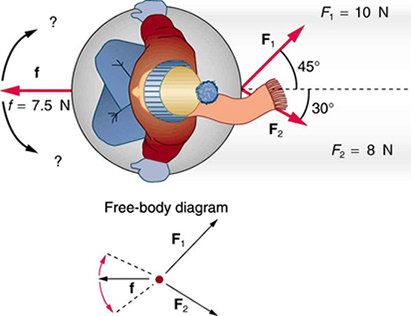
\includegraphics[width=0.4\textwidth]{child.jpeg}
\caption{\label{fig:1} A child is pulled by two other children on a sled atop some ice.}
\end{figure}
\end{enumerate}

\end{document}